\documentclass{article}
\usepackage{graphicx}

\title{Pascal’s Phenomenal Triangle}
\author{Cecilia Sun}

\begin{document}

\maketitle
Everyone knows about Pascal’s peculiar triangle --- start with a row (this will be row $0$) containing just a $1$, then for each entry in the subsequent row, add the two numbers directly above it, where we treat a blank entry as a $0$, and continue iterating downwards forever. The first eight rows look like this:
\[\begin{array}{c}1\\1\quad 1\\1\quad 2\quad 1\\1\quad 3\quad 3\quad 1\\1\quad 4\quad 6\quad 4\quad 1\\1\quad 5\quad 10\quad 10\quad 5\quad 1\\1\quad 6\quad 15\quad 20\quad 15\quad 6\quad 1\\1\quad 7\quad 21\quad 35\quad 35\quad 21\quad 7\quad 1\end{array}\] %copied from wikipedia, lmao

Pascal’s playful triangle has enthralled mathematicians all over the world for centuries, and for good reason --- there are all sorts of patterns and mysteries encoded in this pretty-famous triangle! Here are just a few:

\textbf{Picking things}

Recall that the binomial coefficient 
\[
	\binom nk
\]
is the number of ways to choose $k$ things out of $n$. 

It turns out that the entry in $n$th row and $k$th column (where we start indices from $0$) is precisely $\binom nk$.

Because we get each entry by adding the two entries on top of it, we can now deduce \textit{Pascal's identity}:

\[\binom nk=\binom{n-1}{k-1}+\binom{n-1}k.\]

\textbf{Paths}

Say I have a pet ant named \textit{Ant}hony. 

I place Anthony on the topmost $1$ of the triangle, and instruct him to travel downwards atop the entries: every second, Anthony moves down a row, but he can only move downwards and to the two numbers directly below the number he is currently on.
Then, each number Anthony travels over is precisely the number of paths he could have taken to get there. 

Why is this true? 

Well, for every number, there were two numbers that Anthony could have been at a second before; thus, the number of possible ways he could have gotten to his current number is the sum of those two numbers. Wait\dots This is exactly how we construct Pascal's triangle!

\textbf{Binomial Expansions}

%insert quirky image nvm
When we expand binomials, such as $(x+1)^n$, the coefficients are the entries in the $n$th row of the triangle! 

For example, the expansion of $(x+1)^3$ is 
\[1x^3+3x^2+3x+1,\]

and we can observe that row $3$ of Pascal's triangle is indeed 
\[
	\begin{array}{c}1\quad3\quad3\quad1\end{array}
\]

This is no coincidence! To see why this is true, we can look at how we get the coefficients of $(x+1)^{n+1}$ given only the coefficients of $(x+1)^n$.

Well, we know that
\begin{align*}
	(x+1)^{n+1}&=(x+1)(x+1)^n \\
			   &= x(x+1)^n+(x+1)^n
\end{align*}

In very vague terms, when we multiply $(x+1)^n$ by $x$, we are ``shifting'' the coefficients in the expansion of $(x+1)^n$ to the right by $1$ (since we're increasing each power of $x$ by $1$). Then, we add it back to the ``unshifted'' coefficients to get the coefficients of the expansion of $(x+1)^{n+1}$. 

For example, going from $n=3$ to $n=4$ looks like this:
\[
\begin{array}{c|ccccc}
\text{coeffs of } x(x+1)^3 & &1&3&3&1 \\
\text{coeffs of } (x+1)^3 & 1&3&3&1& \\
\hline
\text{coeffs of } (x+1)^4 & 1&4&6&4&1
\end{array}
\]

It looks like we're really just adding the adjacent entries of the previous rows to get the new rows\dots This is also how we generate new rows of Pascal's triangle! 

\textbf{Fibonacci's triangle?!}

The Fibonacci sequence is also hidden in Pascal's triangle! Let's move all the entries to the left, then sum each diagonal, as so:

\begin{center}
	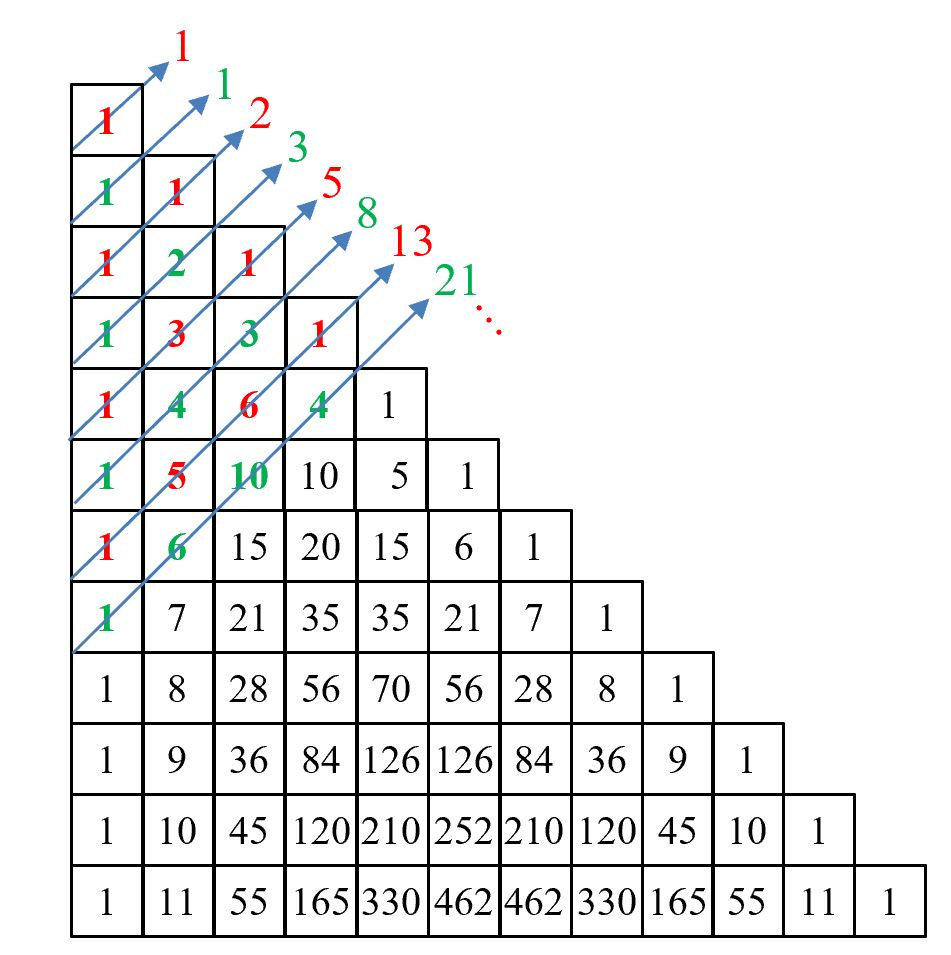
\includegraphics[width = 2 in]{images/pascal1.png}
\end{center}

When we sum the diagonals, we end up with the Fibonacci sequence! 

Remark: Written more formally, this fact is saying that
\[\sum_{k=0}^{\lfloor n/2\rfloor}\binom{n-k}k=F_{n+1}.\]
If you're comfortable with induction and summations, you might want to try proving this\footnote{Pascal's identity may be handy here.}!


\textbf{Sierpinski's triangle?!}

What happens when we color all the odd numbers in Pascal's triangle? It turns out, we get something that looks like Sierpinski's triangle! 

\begin{center}
	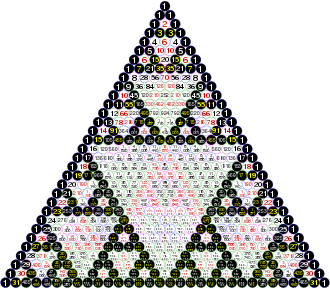
\includegraphics[scale=0.45]{images/pascal2.png}
\end{center}

And as we extend further and further downward, we get closer and closer to Sierpinski's triangle.

Things get even more interesting when we color every number based on their remainder when divided by different numbers. 

If we color based on their remainders when divided by $3$, $4$, and $5$, we get the following patterns. All of these images were taken from the \href{https://www.maa.org/press/periodicals/loci/joma/patterns-in-pascals-triangle-with-a-twist-first-twist-what-is-it}{MAA}:


\begin{center}
	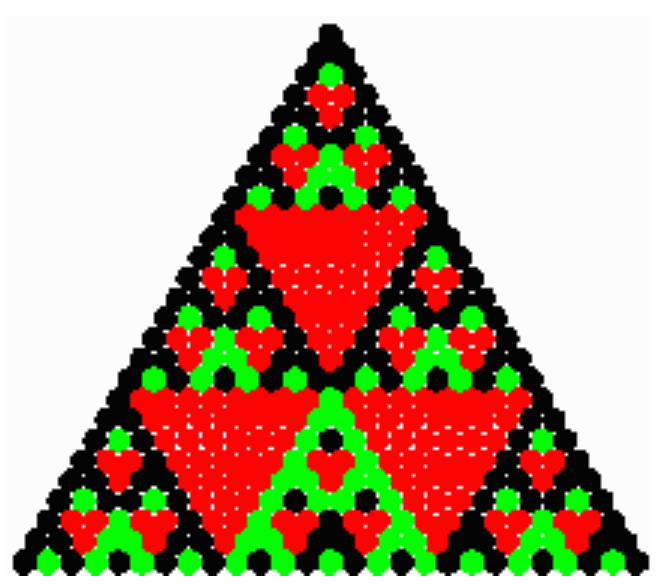
\includegraphics[scale=0.35]{images/pascal3.png}
\end{center}

\begin{center}
	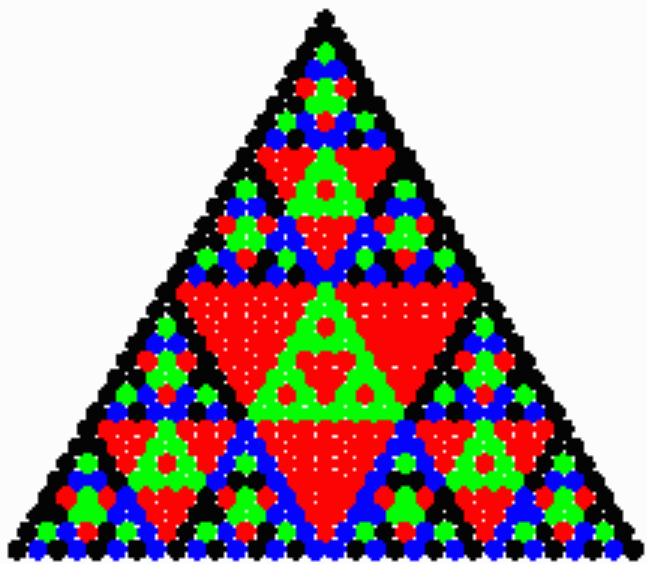
\includegraphics[scale=0.35]{images/pascal4.png}
\end{center}

\begin{center}
	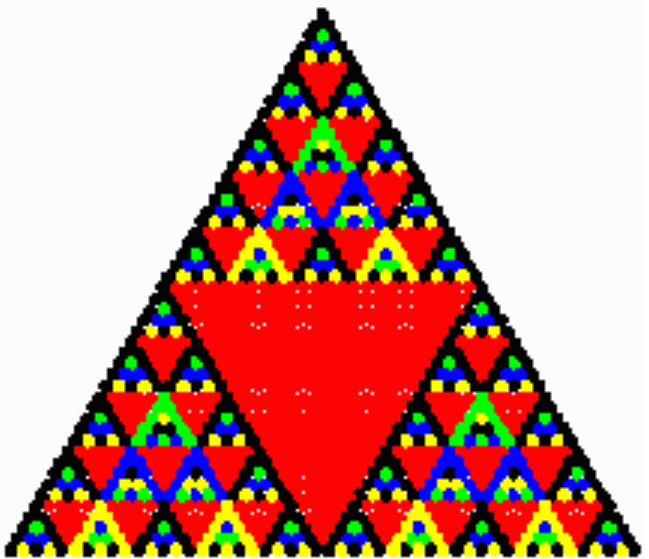
\includegraphics[scale=0.35]{images/pascal5.png}
\end{center}


Those were just some of the patterns in Pascal's popular triangle. Perhaps if you're patient, persistent, and play around a bit, you'll find even more!
\end{document}